% Name: Atwood machine
% Description: Two masses hanging from one rope over a fixed pulley, with the tension and the weight on each and the way they accelerate.
% Tags: pulley, Atwood machine, tension, acceleration

\usetikzlibrary{arrows.meta, patterns}

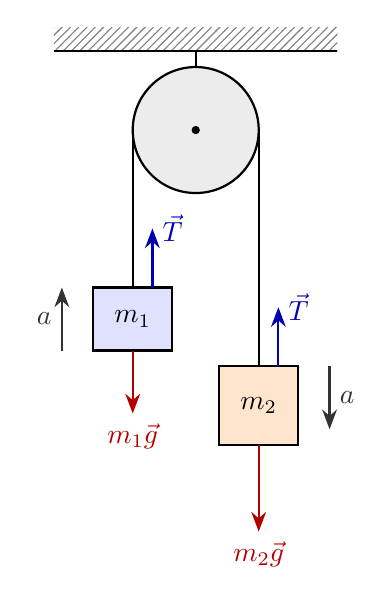
\begin{tikzpicture}[>={Stealth[length=2.5mm]}, force/.style={->, thick}]
  \fill[pattern=north east lines, pattern color=gray] (-1.8,4.2) rectangle (1.8,4.5);
  \draw[thick] (-1.8,4.2) -- (1.8,4.2);
  \draw[thick] (0,4.2) -- (0,3.2);
  \draw[thick] (-0.8,3.2) -- (-0.8,1.2);
  \draw[thick] (0.8,3.2) -- (0.8,0.2);
  \draw[thick, fill=gray!15] (0,3.2) circle (0.8);
  \fill (0,3.2) circle (1.5pt);
  \draw[thick, fill=blue!12] (-1.3,0.4) rectangle (-0.3,1.2) node[midway] {$m_1$};
  \draw[thick, fill=orange!20] (0.3,-0.8) rectangle (1.3,0.2) node[midway] {$m_2$};
  \draw[force, blue!70!black] (-0.55,1.2) -- ++(0,0.75) node[right] {$\vec{T}$};
  \draw[force, blue!70!black] (1.05,0.2) -- ++(0,0.75) node[right] {$\vec{T}$};
  \draw[force, red!70!black] (-0.8,0.4) -- ++(0,-0.8) node[below] {$m_1\vec{g}$};
  \draw[force, red!70!black] (0.8,-0.8) -- ++(0,-1.1) node[below] {$m_2\vec{g}$};
  \draw[->, thick, gray!40!black] (-1.7,0.4) -- ++(0,0.8) node[midway, left] {$a$};
  \draw[->, thick, gray!40!black] (1.7,0.2) -- ++(0,-0.8) node[midway, right] {$a$};
\end{tikzpicture}
